
\section{Results}
\noindent Figures \ref{f_singlepar}, and \ref{f_multipar} show 9 skateboard shapes that have improved ollie height compared to the industrial standard Popsicle stick skateboard geometry (Base in figure \ref{f_nopar}) when optimized for optimal ollie height. The best performing skateboard shape (number 2 in figure \ref{f_multipar} improved ollie height by 11.1 \%. All optimizations are with a null seed initial guess and solved with an optimal IPOPT exit status with the desired NLP tolerance and mesh tolerance found in \ref{s_settings}. All optimizations were solved within 3 minutes. Four skateboards did not show improvement in ollie height, which are indicated with a red dot. These are per definition local maxima, because the base optimization is a higher solution, which is in the solution space of these optimizations. 

\subsection{Optimal Trajectories and \\Geometries}
\subsubsection{No parameter optimization}
\begin{figure*}
    \centering
    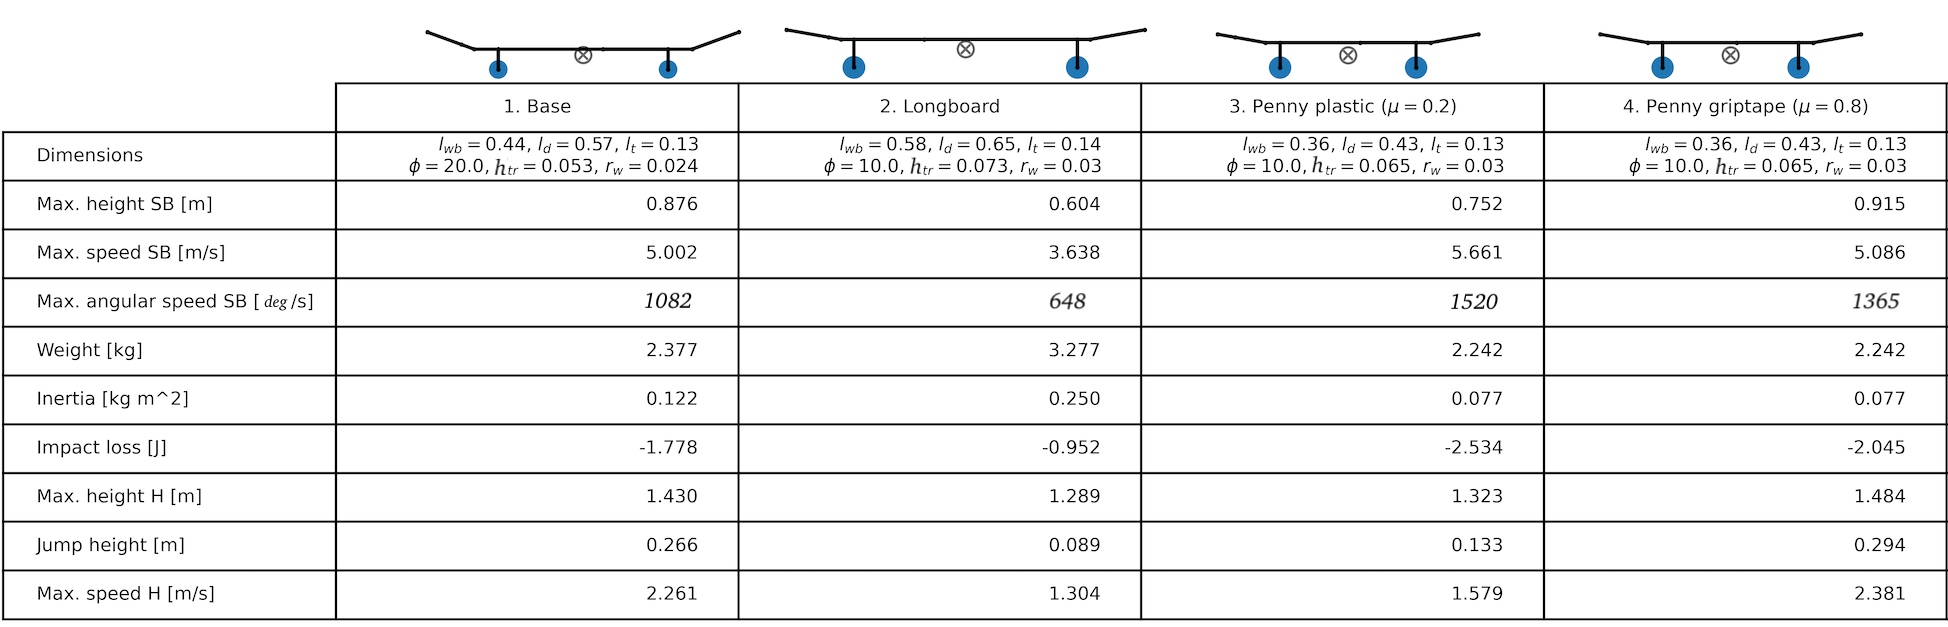
\includegraphics[trim={0 0 0 0},clip,width=\textwidth]{figure/Results/no_optimization_table_dpi600.png}
    \caption[Optimal control  benchmarks for ollie without parameter optimization]{Optimal control benchmarks for ollie without parameter optimization - Schematic skateboard set-ups used to find the optimal ollie. The table shows important benchmarks. Jump height is calculated by minimum vertical position minus take-off vertical position of the person. The impact loss is calculated with kinetic energy of the skateboard after impact minus kinetic energy of the skateboard prior to impact. Other variables are direct output from optimization. }
    \label{f_nopar}
\end{figure*}

\noindent The no parameter optimization was done test the real life scenario that a long board and a penny board are more difficult to ollie. The longboards' dimension are set to an arbitrary OEM longboard.\footnote{\url{https://hlcskateboardfactory.com/ shape: MB701}} The penny boards' dimensions are set to an arbitrary penny board. A penny board is usually made from plastic.\footnote{\url{https://skateboardelite.com/what-is-penny-board/}} The coefficient of friction for the plastic penny is set to 0.2 \cite{bani-hani_data_2019}. For a comparison if the shape of a penny could actually ollie higher a version with griptape is also shown. The three boards are optimized to verify the optimization. Longboard complies with the real life scenario and the optimization shows a 31\% decrease in ollie height compared to the base . The penny board with a plastic top (lower coefficient of friction) is able to ollie 14.2\% lower than the base.

The base skateboard is able to ollie 31\% higher than the long board. The longboards' maximum angular velocity is 40.0\% lower compared to the base skateboard. This is probably due to the fact that the inertia and mass of the long board are higher which will make it harder for the human with limited power to rotate it and get it up. The jump height of the human on the long board is 66.5\% lower compared to the base, meaning that a lot of power is going into the long board instead of jumping up. Resulting in the human mainly to tuck in without jumping). The impact loss is lower for the long board. This could be correlated to the fact that it reaches lower speeds. The contrary is seen with the plastic penny board. It reaches higher speeds and loses more energy during impact. The penny boards are 5.7\% lighter than the base board but have a lower inertia mainly due to the smaller size of the penny board. With a plastic penny board, the human is not able to ollie higher than with the base skateboard. The human jumps 50.0\% and ollies 0.124 [m] lower with the plastic penny board. With grip-tape the penny board is able to ollie higher than the base skateboard. In real life the penny board and long board are harder to ollie. The same is shown in the optimization for the long board. This suggests that the kinetics of the optimization are similar to reality. The penny with griptape is able to ollie higher than the base skateboard, which could have multiple causes. One of them is that a real penny board is made of plastic which deforms more than wood. Which could cause more dissipation of energy and a more difficult control to ollie. The other cause could be that the optimization is lacking kinematic constraints for the human. In real life it is harder to maintain balance when your feet are in a narrow stance. During the balancing narrow stance, in real life it could be more difficult to exert maximal leg power.

\subsubsection{Single parameter optimization}

\begin{figure*}[t]
    \centering
    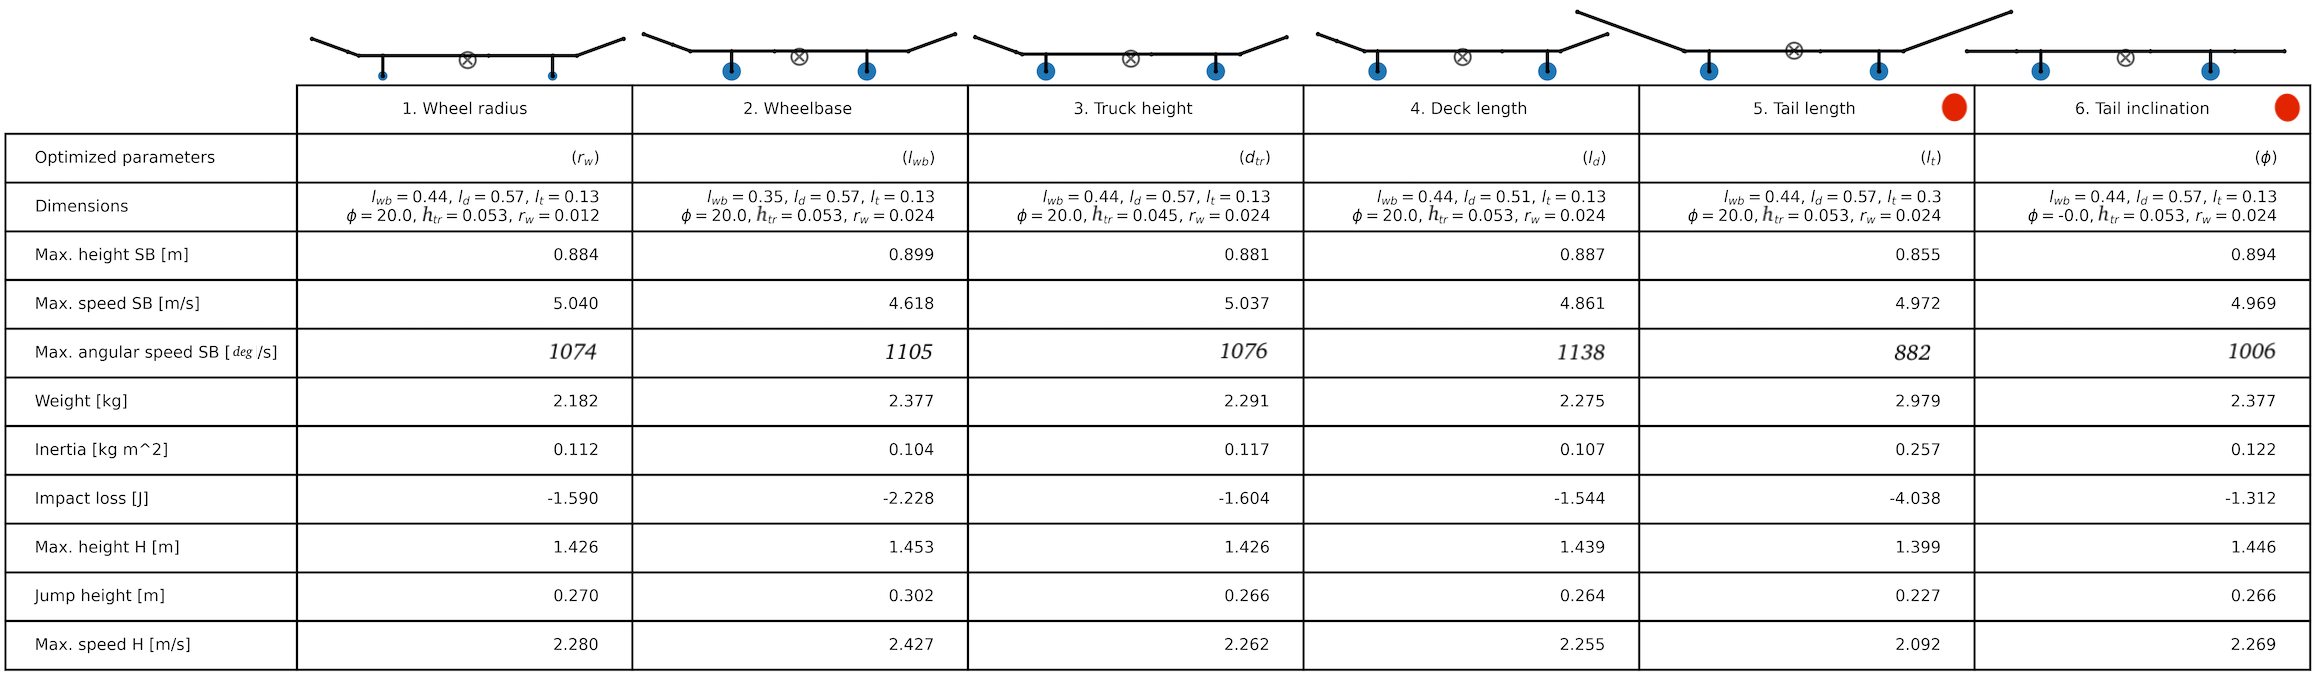
\includegraphics[trim={0cm 0cm 0cm 0cm},clip,width=\textwidth]{figure/Results/single_optimization_table_dpi600.png}
    \caption[Geometry solutions and benchmarks for single parameter optimization]{Geometry solutions and benchmarks for single parameter optimization. The best performing optimization is 2, where the wheelbase is optimized.}
    \label{f_singlepar}
\end{figure*}
\noindent All single parameter optimizations are visible in figure \ref{f_singlepar}. Compared to the base skateboard, all single parameter optimization skateboards were able to ollie higher except for the tail length optimization. The difference in ollie height between the base and the single parameter optimizations is minimal (0.05-0.023 [m]) which suggests that the base skateboard is very close to it's optimum when only one variable can be changed. All single parameter skateboards except for the wheelbase and tail length optimizations show similar human jump height. Which indicates that with these configurations the human is able to exert similar power over time. With a smaller wheelbase the human was able to jump higher. The main differences are found in the weight and inertia reduction which could be the main `drive' of the single parameter optimization. Geometrically the optimizer isn't able to find a large ollie improvement as seen between the base and long board. Still, the optimizer can find a higher optimum by decreasing weight and inertia with all single parameter optimizations except for the tail length and tail inclination optimizations. Which indicates that inertia and weight reduction is a positive influence for ollie height. Dynamically this makes sense because with lower mass and inertia values it easier to lift and rotate the skateboard. The wheel radius, truck height, and tail inclination are hitting the bounds of 0.0125[m], 0.045[m], and 0[deg] respectively, which may indicate a local maxima. Also the tail length optimization did not find a higher maxima than the base optimization which makes it a local maximum per definition, because the base skateboard is a possible solution for this optimization.

\subsubsection{Multiple parameter optimization}
\begin{figure*}
    \centering
    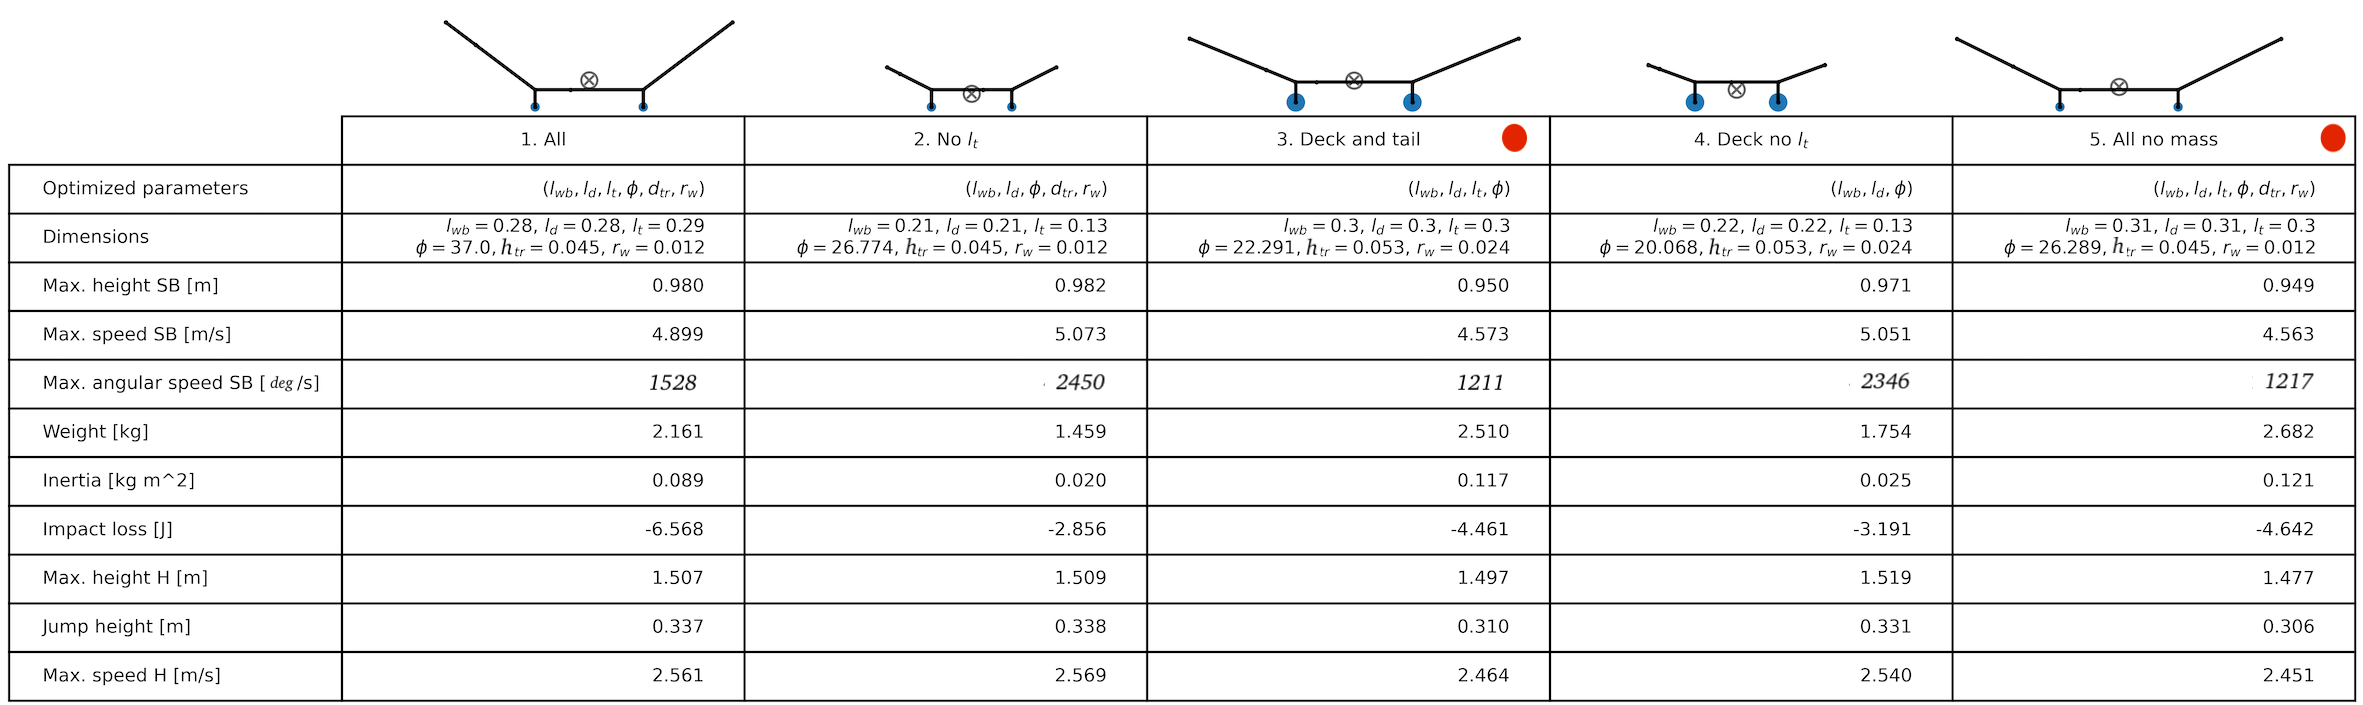
\includegraphics[trim={0cm 0cm 0cm 0cm},clip,width=\textwidth]{figure/Results/multi_optimize_table_dpi600.png}
    \caption[Geometry solutions and benchmarks for multiple parameter optimization]{Schematics of multiple parameters optimizations. Table shows important benchmarks.}
    \label{f_multipar}
\end{figure*}

\noindent All multiple parameter optimizations are visible in figure \ref{f_multipar}. When multiple parameters are optimized the ollie height is improved by 0.074-0.106 [m] compared to the base skateboard. The first column, 'All' in figure \ref{f_multipar} shows the set-up when all parameters are optimized. As seen with the single parameter optimization the tail length is causing strange optima. Once again it is shown that when not optimizing the tail length, the ollie height is higher. This proves that the optimization of all variables is a local optimum, since the optimum found with the `no $l_t$' (figure \ref{f_multipar}) skateboard is a possible solution to the optimization. Same goes for the full deck optimization. The full deck optimization does not optimize wheel radius and truck height. The ollie height for this optimization is 0.021 [m] lower than the same optimization with fixed tail length. This proves that the full deck optimization is a local maxima which is caused by the optimization of the tail length. The cause of hitting a local optimum because of the tail length needs further investigation. When the tail length increases the impact loss increases as well. This is logical when thinking of the tail speed $v = \omega \times r$, which means, the larger the distance between the tip of the tail and COM of the skateboard, the larger the local speed at the tail. The larger the speed at the tail, the more momentum is lost during impact, which is the reason for the higher impact losses. The impact loss is dependant on the mass and speed, the higher the mass or the speed, the higher the impact loss will be. For example in the `no $l_t$' (figure \ref{f_multipar}) optimization the angular velocity before impact is more than twice as high compared to the base optimization. But the mass is also 0,878[kg] less. Thus, the large angular velocity causes the impact loss to be higher, but the mass reduction reduces it, only causing a slight gain in impact loss. 

The most promising optimizations are analyzed further by looking into the states and control over time and compared to the base optimization. The single parameter optimizations show little improvement. The best performing single parameter optimization is the wheelbase optimization with an increase of 2.6\%. The best performing multiple parameter optimization are `no $l_t$' (figure \ref{f_multipar}) (12.0\% increase in ollie height) and deck without tail length (10.7\% increase in ollie height).  All other detailed figures of the optimizations are found in Appendix A. 
\begin{figure*}
    \centering
    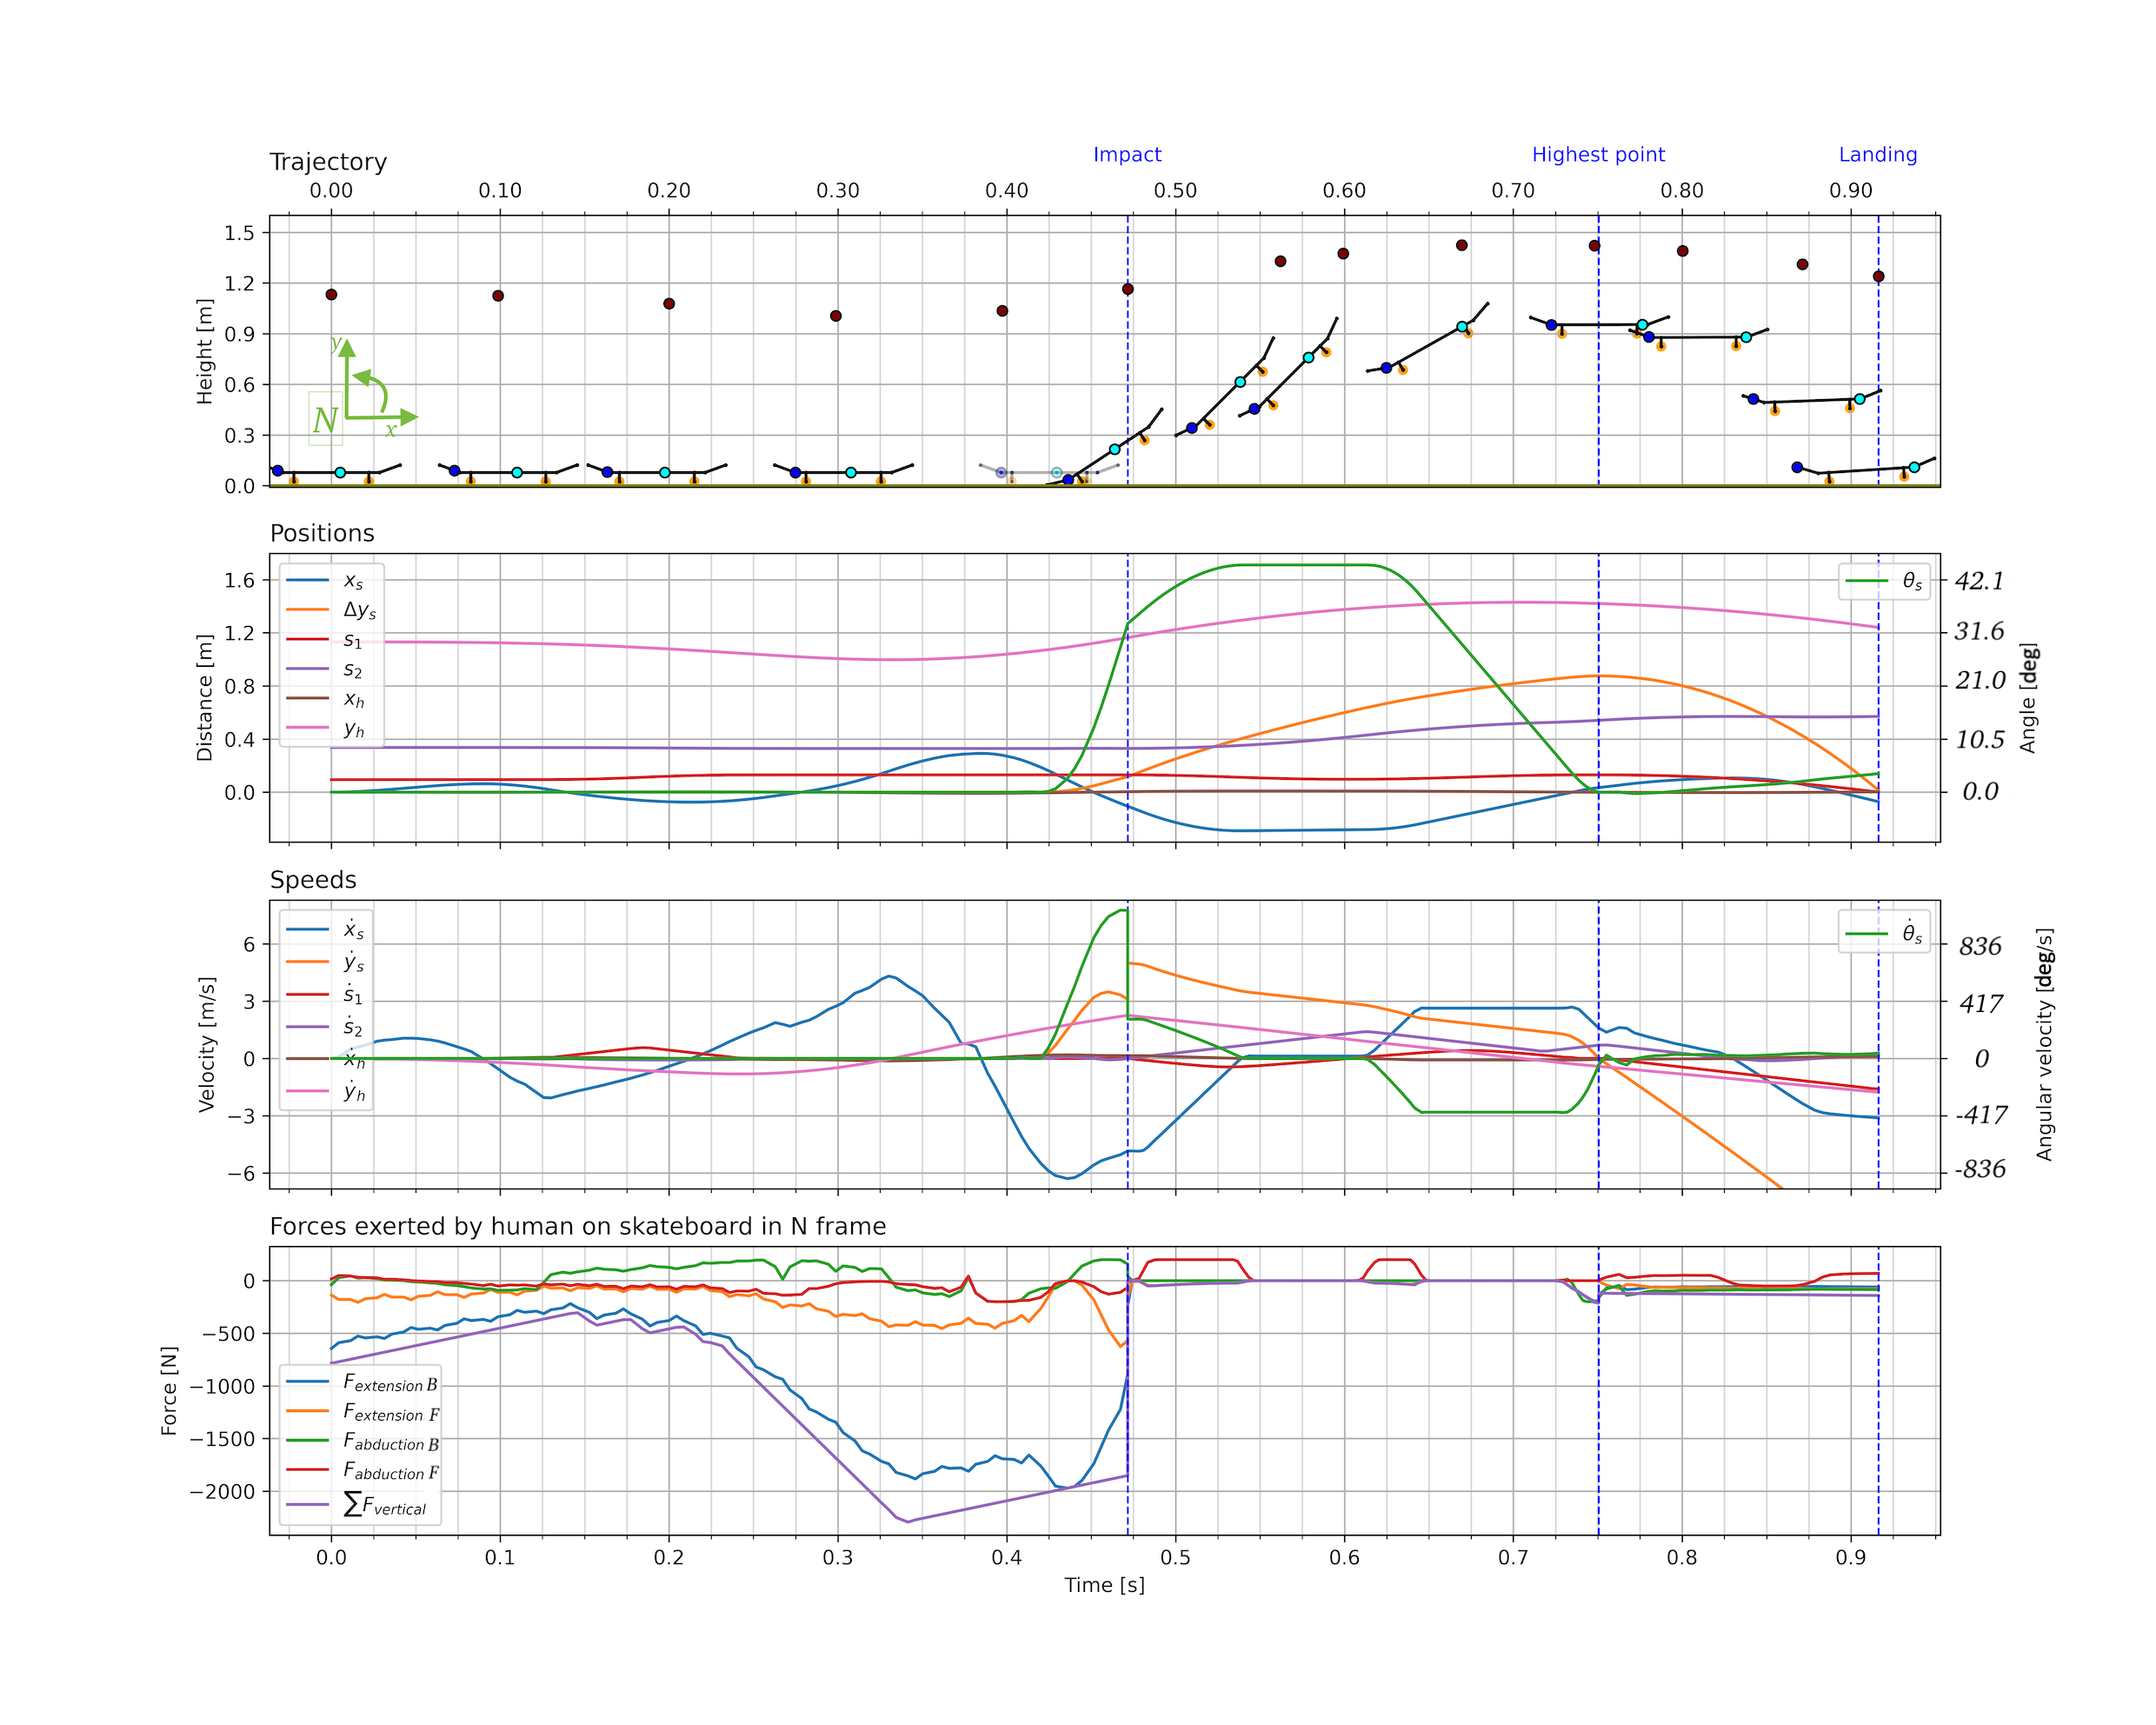
\includegraphics[trim={0cm 0cm 0cm 0cm},clip,width=\textwidth]{figure/Results/data_basedpi600.png}
    \vspace{-1.5cm}\caption[Trajectory, positions, speeds, and forces of base optimization]{Optimization of base skateboard. Corresponds to results in figure \ref{f_nopar}.1. Graph (1) shows the trajectory of the skateboard, (2) are the positions, (3) are the speeds, (4) are the forces. The blue dotted lines are the phase switches. First the human lowers their COM (pink,2) by decreasing vertical force (purple, 4), at minimal human COM height there is maximal force and zero speed (pink,3). Maximal force is almost fully caused by the extension force of the back foot (blue,4). Speed is increased until impact and it reaches maximum speed (pink,3 at impact). Just before impact the skateboard rotates its angle (green,2) from 0 to impact angle. Mid air the speeds are constant except ones effected by gravity (orange,pink,3). The moments forces are exerted the velocities change (t=0.5, t=0.63). The human reaches its highest point before the skateboard. At the highest point force is exerted to `catch' the skateboard. Landing is achieved by stretching and landing on the back wheel }
    \label{f_noparameter}
\end{figure*}
\subsection{Detailed trajectories}
\noindent The results of the optimizations are presented stacked vertically with a shared x-axis which represent time in figures \ref{f_noparameter}, \ref{f_wheelbase}, \ref{f_notail}, and \ref{f_notailnotruck}. The top plots in these figures are the trajectories shown with snapshots at certain time increments. The human centre of mass corresponds with the time of the snapshot. The phase switches are indicated with the blue dotted lines. The positions of the back and front feet are indicated with the dark blue and light blue dot respectively. The second and third plots in these figures are the positions and the velocities respectively. The bottom plots show the forces exerted by the human acting on the skateboard. All states and forces are expressed in the N-frame convention visible in the left corner of the trajectory. The angle and angular velocity are expressed on a second vertical axis at the right of the figures because the units are different from the rest of the states. The forces are presented with the extension force and abduction force. The extension forces correspond to N-frame y direction and abduction forces act in N-frame x-direction as explained in section ref{}. The blue line corresponds to N-frame y-direction leg force acting between the center of mass (red dot in trajectory figure) and the back foot (blue dot in trajectory figure), while the orange line corresponds to the N-frame y-direction leg force acting between the center of mass and the front leg (cyan dot in trajectory figure). The abduction forces are the forces acting between the feet and the COM in N-frame x-direction. For example, before impact, both legs are pushing vertically down on the board, after impact the front foot is pushing sideways in positive x-direction. The sum of the N-frame y-axis forces is presented as the purple line. To see all trajectories that will be presented in the following paragraphs with forces as a video, visit: \url{https://www.youtube.com/watch?v=jw5DmNnvD7c}. In the video static friction and dynamic friction are shown to be performing properly.


\subsubsection{Base skateboard optimization}


\noindent The first figure concerns the optimal control problem without parameter optimization shown in figure \ref{f_noparameter}. The trajectory is very similar to the trajectory seen in figure \ref{f_olliesteps}. Though you have to take into account that this ollie is a standing ollie without an initial horizontal velocity, whereas figure \ref{f_olliesteps} shows a riding ollie. The skateboard relative to the human first moves forward, and just before the impact it rapidly moves backward followed by the tail hitting the ground. The backwards movement happens such that the human can effectively pull the skateboard up and forward with friction and perpendicular force which results in the skateboard being straight under the human at the highest point. The backwards velocity is clearly visible in fig. \ref{f_nopar} speeds, where the blue line before impact is at the largest negative velocity. After impact the velocity will gradually become positive and ending at an almost 0 x position of the skateboard (blue line in positions at second dotted line). If there would not have been a backwards movement, the skateboard would have been pushed out of reach of the human's feet when the board is leveling out. The skateboard is leveled out by a positive abduction force of the front foot (red line forces at $t=0.47-0.55$ and $t=0.62-0.65$). These forces result in a decrease in angular rotation (green line speeds, same time span), and a level skateboard at the highest point (green line positions at highest point = 0).
You can see that the back foot is almost fully located at the pocket of the skateboard. This is the point with the lowest velocity of the tail, the tip of the tail has the highest velocity due to $v = \omega \times r$. When the board is rotating the power that can maximally be exerted by the human legs is limited by the force and the relative velocity: $P_{leg} = v_{rel} F$. This means that if the intention is to jump up as high as possible, the relative speed should be as low as possible, which is why the foot should be in the pocket. When the foot would be on the tip, more distance is lost which could have resulted in a higher jump. 
The impact changes the momentum of the skateboard. In the speeds graph it is visible that the angular velocity at impact vastly reduces (green line, 1082 to 286 [deg/s]), whilst vertical velocity is gained (orange line, 3 to 5 m/s).
The human starts with their knees slightly bent, and having full body weight on the skateboard. In the first phase the human lowers their COM in order to prepare the legs to jump. This is called the unloading phase (from $t=0 - 0.2$). After the unloading phase the force increases. Here the human is braking the downward velocity gained during the unloading phase up until the highest peak of the sum of the vertical forces (purple line). This is called eccentric braking. Then the human vertical velocity (pink line speeds) is at 0 and the human has reached its lowest point. From $t=0.35$ until impact the human is gaining upward speed  (pink line speeds) and reducing the force. The force needs to reduce to comply to the power bound ($P_{leg} = v_{rel} F$). This phase is called the concentric phase. Then the human has lost contact from the skateboard just after impact. Followed by an upward motion gradually decreasing due to gravity, reaching it's highest point just before the skateboard reaches it's highest point. The slopes and maximum of the vertical forces (purple line) are bound by the eccentric RFD(negative) and concentric RFD(positive) and the maximum force permitted. The optimizer is at the bounds and wants to maximize force and power output. The forces are not fully smooth due to the fact that the bounds are on both legs, thus simultaneous counteracting of forces between the front and back leg is permitted in the optimization. Having more kinetic data on single legs could improve this. Also the polynomial to estimate the solution used by the software is not plotted correctly here, so the line should be smoother when using the polynomials used per mesh section provided by the software. Due to practical implications this has not been done. The third reason why the control can be less? smooth is due to the friction constraints. These constraints are difficult to solve and are demanding for the optimizer, which sometimes results in non-smooth forces.
The landing is slightly on the back wheels and the human is almost fully stretched out when landing.

\newpage
\subsubsection{Wheelbase optimization}
\begin{figure*}
    \centering
    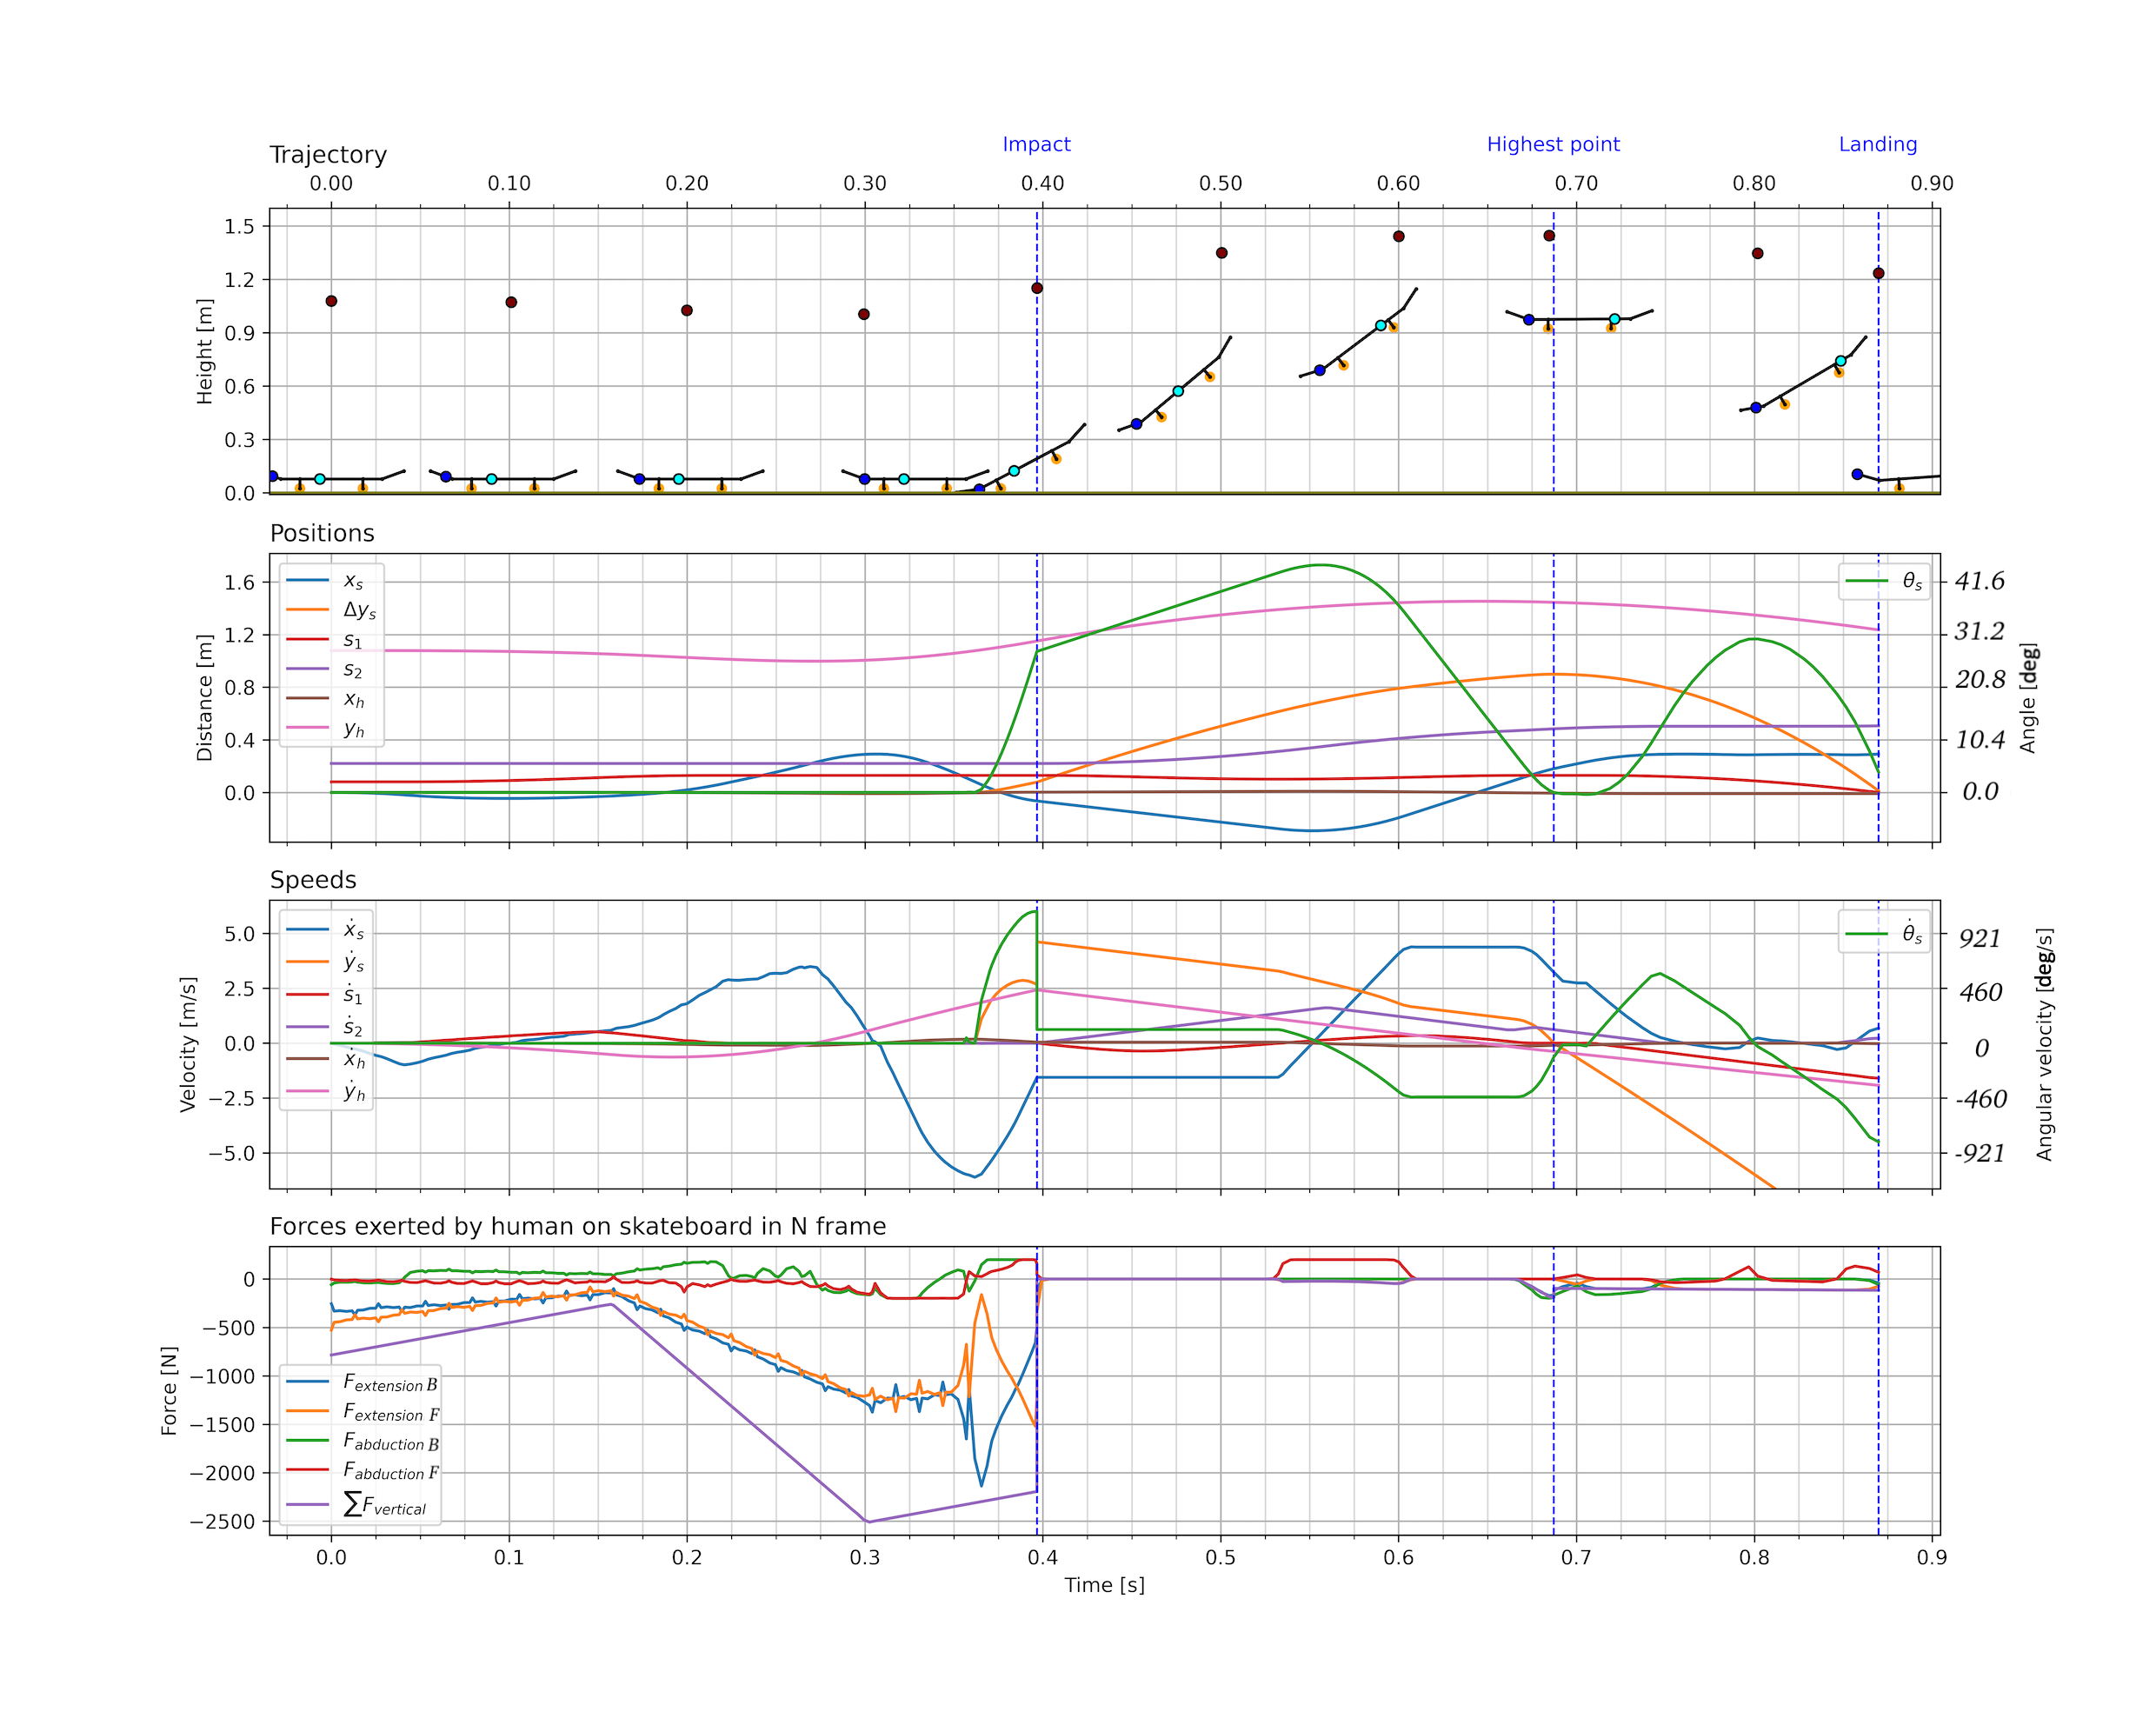
\includegraphics[trim={0cm 0cm 0cm 0cm},clip,width=\textwidth]{figure/Results/data_l_wbdpi600.png}    \vspace{-1cm}\caption[Trajectory, positions, speeds, and forces for wheelbase optimization]{Optimization of wheelbase. Corresponds to results in figure \ref{f_singlepar}.2. 0.09[m] smaller wheelbase compared to base, 0.023[m] higher ollie. Three striking differences, the first is that the jumping force is now equally dependant on the back and front extension force (blue,orange,4), the second is that there is only one force peak between impact and highest point. The third striking part is that the skateboard rotates before landing (t=0.8).}
    \label{f_wheelbase}
\end{figure*}
\noindent The next optimization concerns the single parameter optimization shown in figure \ref{f_wheelbase}. The wheel base of the skateboard will be optimized along with optimal control. The performance of this skateboard has been discussed in figure \ref{f_singlepar}. This skateboard was able to ollie 0.023[m] higher than the base optimization. Most of the phenomena seen in the base optimization are also visible for this optimization. The human lowers their weight, pushes the skateboard forward then pulls it backward. Angular velocity is lost during impact (-1193 [deg/s] and vertical speed is gained (green and orange lines speeds). After impact abduction force with the front leg is used to pull the skateboard up and level it out. The first difference is visible in the force plot. The sum of the vertical forces (purple line) does not stagger when unloading. A straight line up, down, and then up is achieved. Secondly, a higher angular velocity is achieved compared to the base. The back foot is once again in the pocket of the board, but now the front foot is at equal distance from the wheel having perfect balance. At this position both legs can exert equal force without rotating the board during eccentric braking ($t=0.15 - 0.3$). Then suddenly shortly before the impact, the front foot (orange line forces) pulls up and the back foot pushes down to create a maximal momentum about the back axis creating a steep sudden increase in angular velocity. The decreased wheelbase causes the impact angle to be lower and the angular velocity near zero just after impact (green lines positions and speeds). This leaves a period of rest such that the skateboard can gain height. While the front foot is in a sliding motion, the foot starts pushing down on the board at t=0.53.  This is almost enough to level the board out at the highest point. But the negative angular rotation caused by this push is caught with the back foot at the highest point making sure the board is leveled. 
The reason why this board can ollie higher is because it needs less control during the upward motion to level the board out and is able to reach higher angular velocities due to reduced inertia. By decreasing the wheelbase, the inertia of the skateboard is decreased. With a decreased inertia, the dynamic response is faster resulting in higher angular velocity with the same amount of torque produced. Also less force is needed to level the skateboard during the upward motion because the same amount of force input will result in a larger angular deflection compared to the base skateboard. 

\begin{figure*}[t]
    \centering
    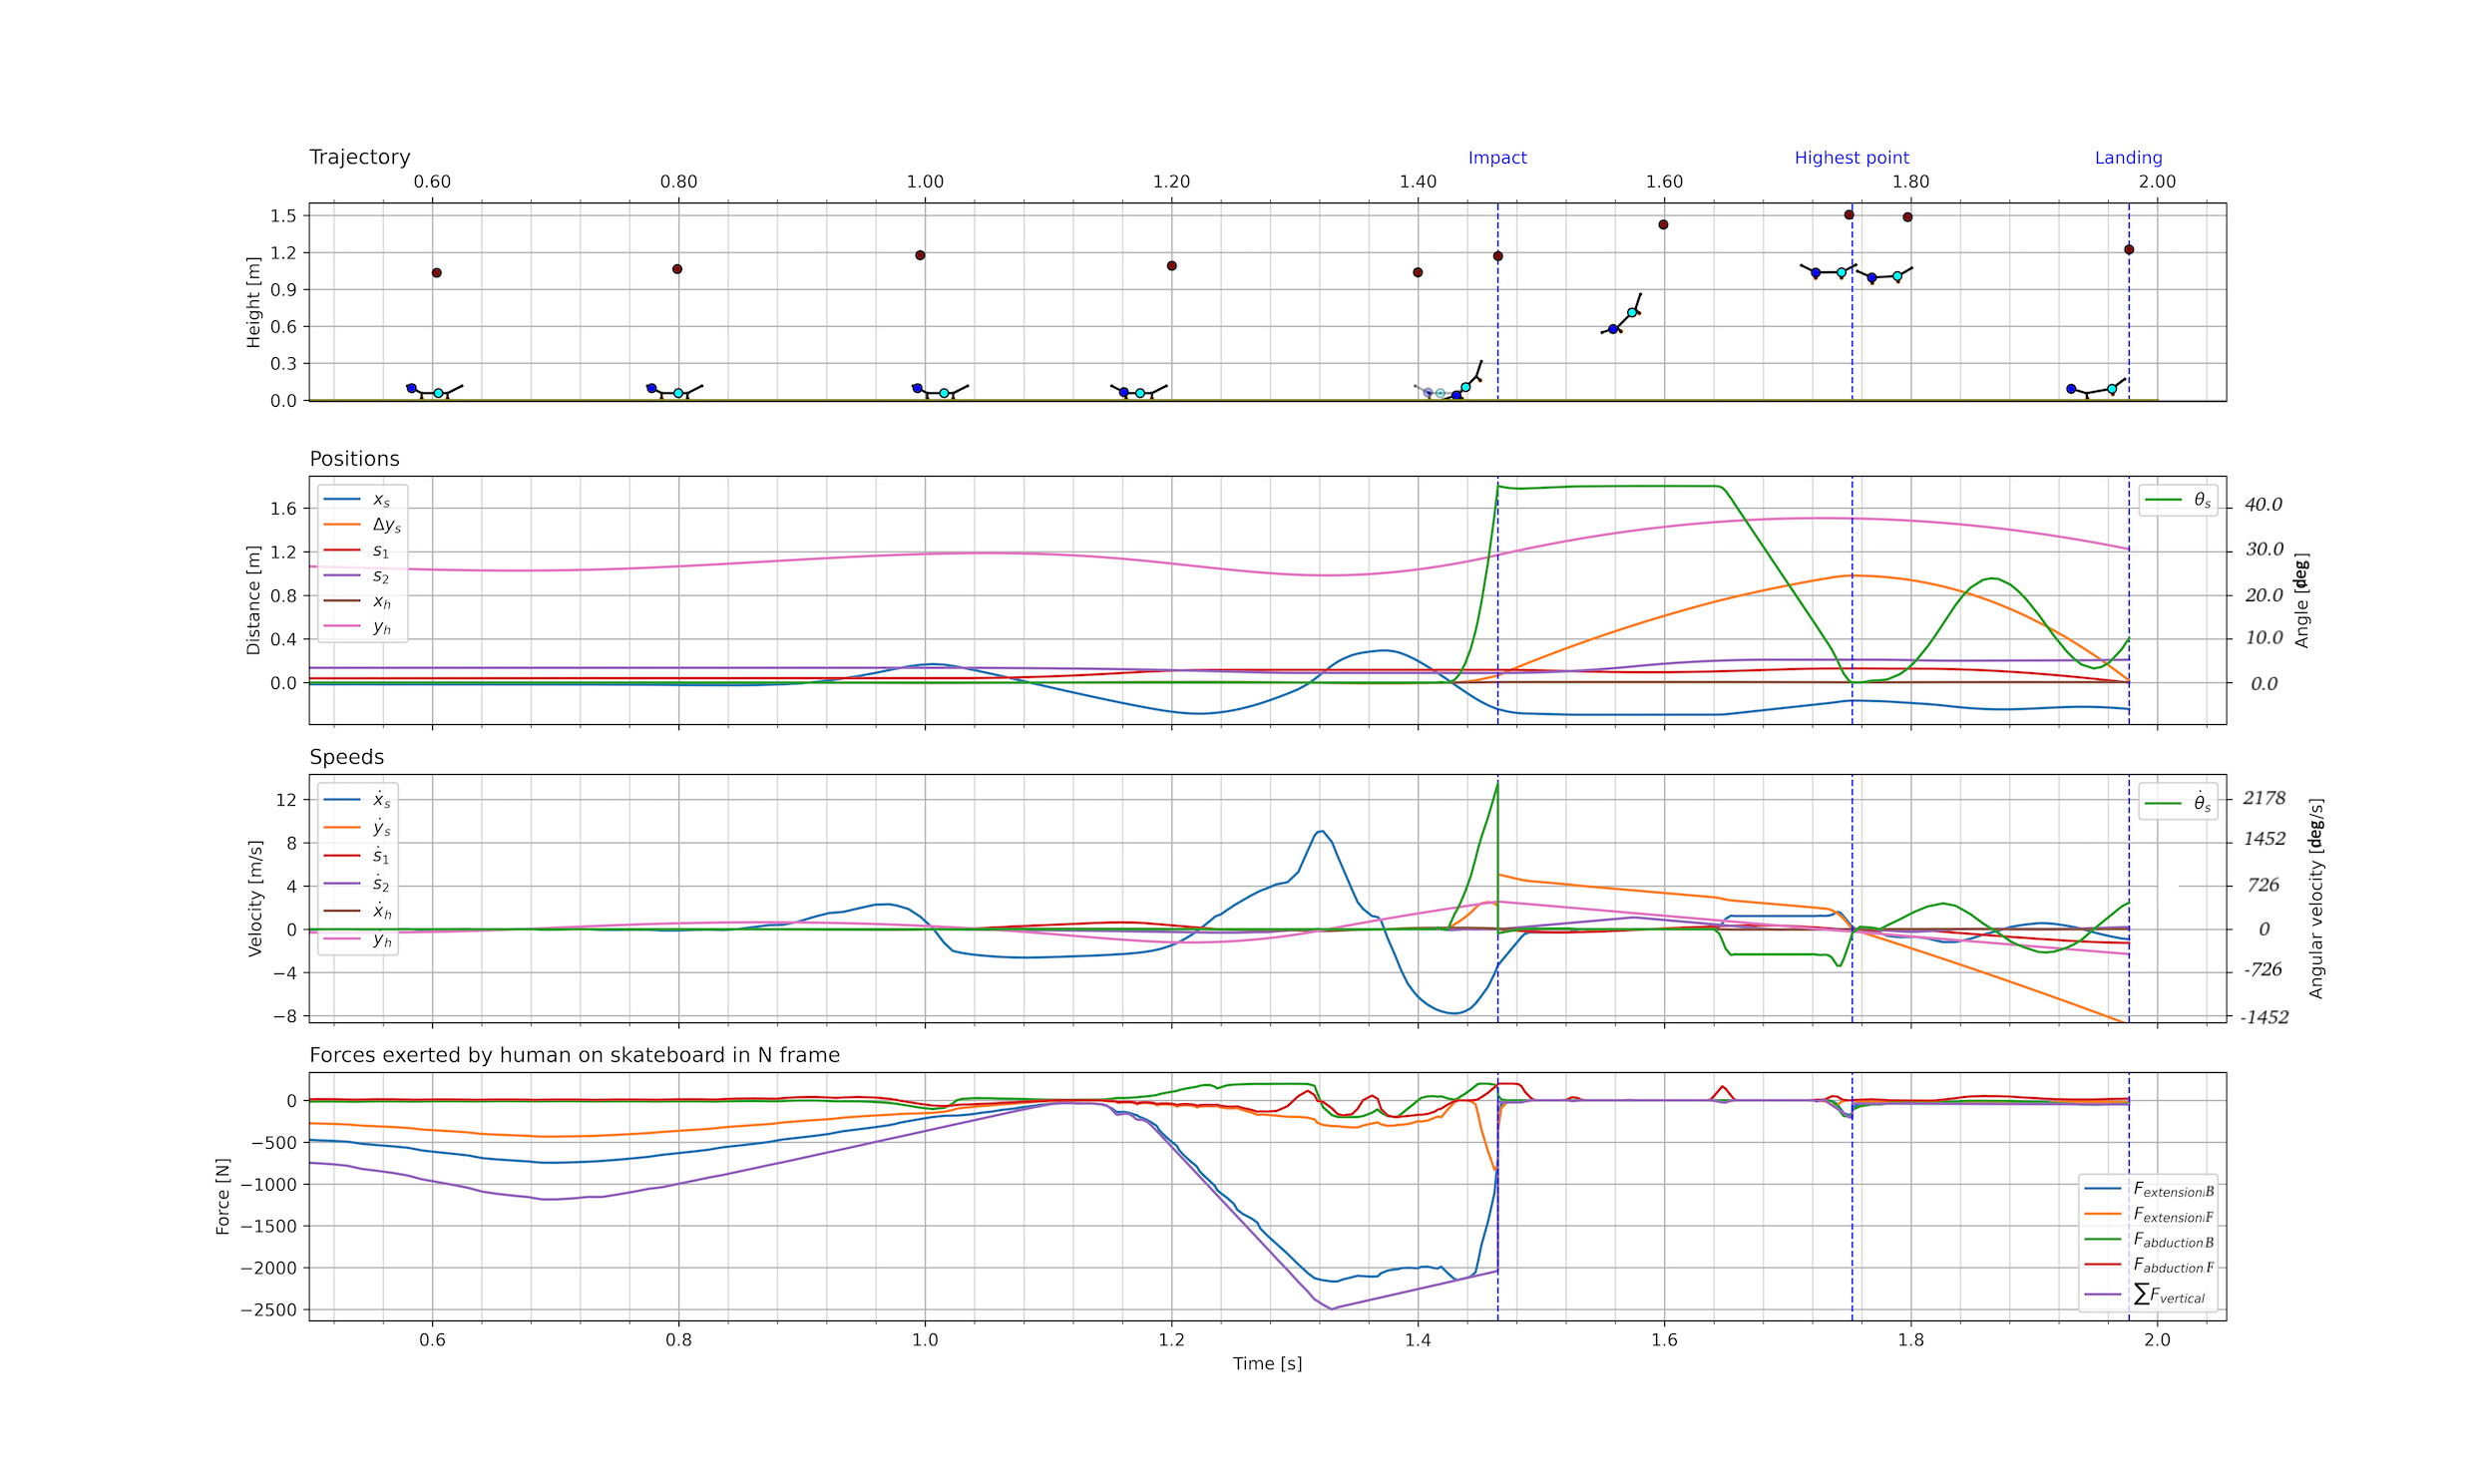
\includegraphics[trim={0cm 0cm 0cm 0cm},clip,width=\textwidth]{figure/Results/data_no_taildpi600.png}
    \caption[Trajectory, positions, speeds, and forces for `all except tail length' optimization]{Optimization `no $l_t$'. Corresponds to results in figure \ref{f_multipar}.2.}
    \label{f_notail}
\end{figure*}
\begin{figure*}[t]
    \centering
    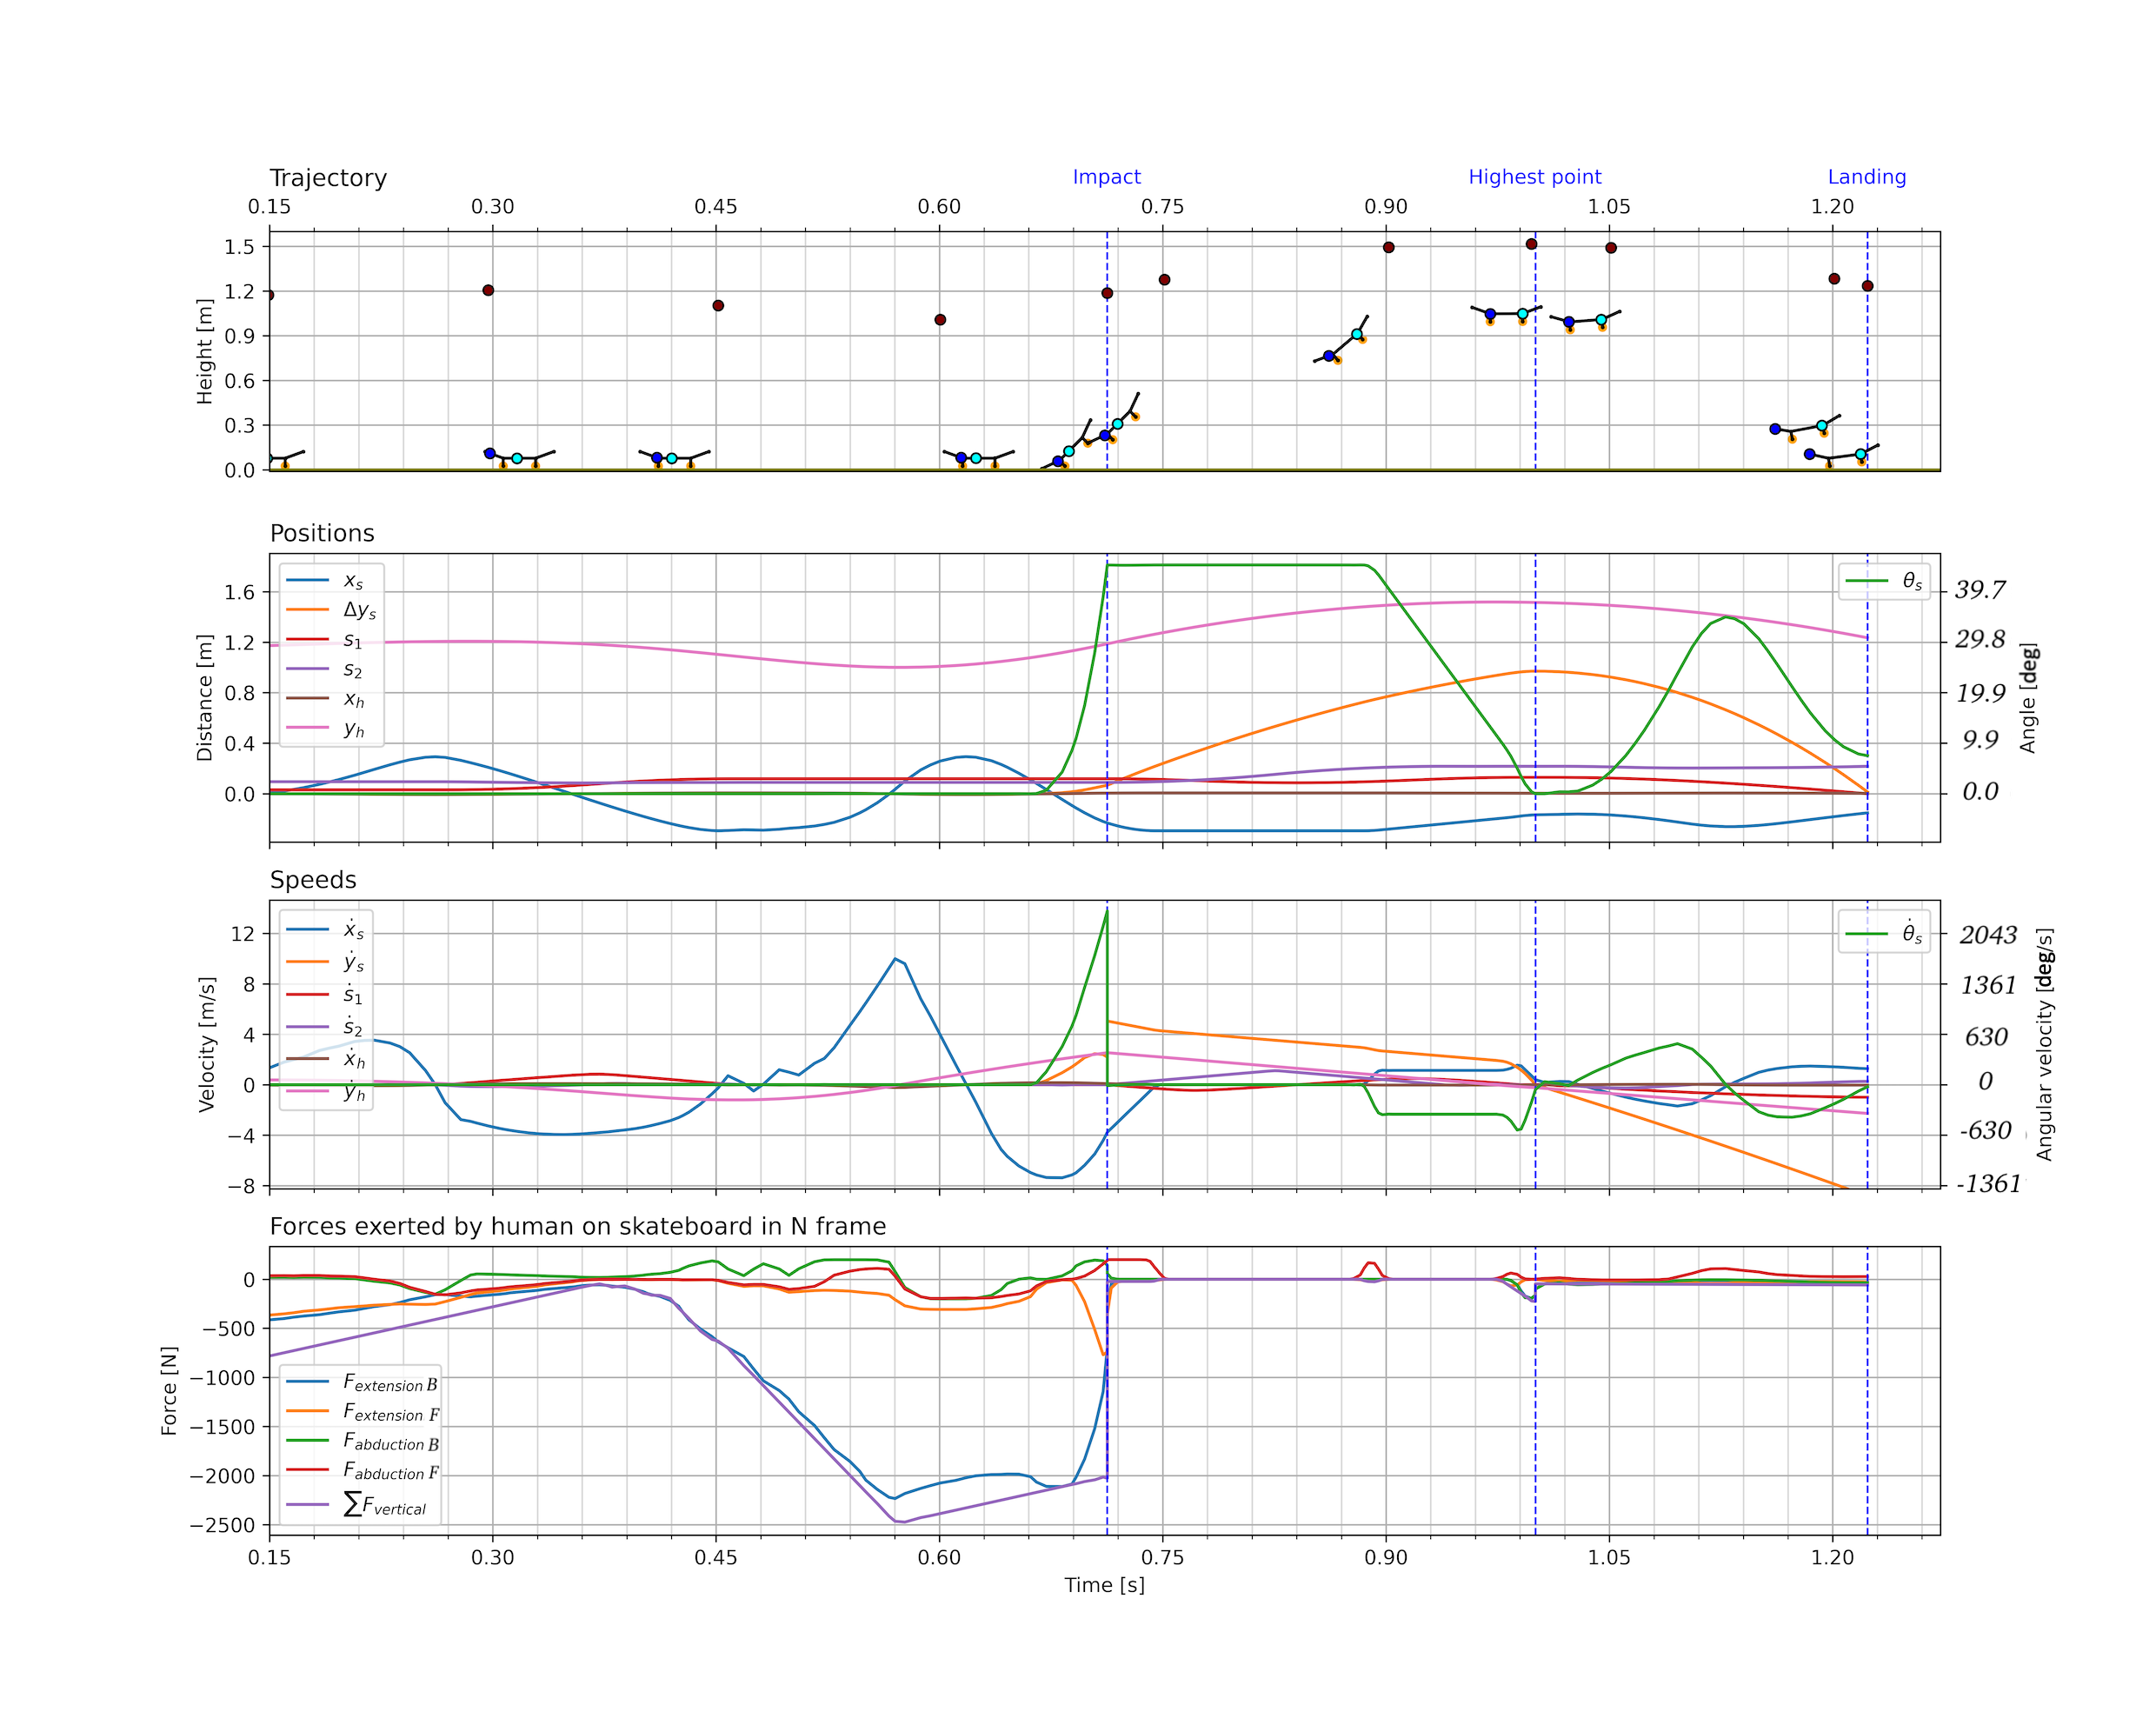
\includegraphics[trim={0cm 0cm 0cm 0cm},clip,width=\textwidth]{figure/Results/data_notrrwltdpi600.png}
    \vspace{-0.5cm}\caption[Trajectory, positions, speeds, and forces for `deck except tail length' optimization]{Optimization `deck no $l_t$'. Corresponds to results in figure \ref{f_multipar}.4. The human first goes up and down before wanting to jump (pink,2). The time before impact is (long 1.46 [s]). The rotational speed at impact is 2178 [deg/s]. Between t=1.5 and t=1.8 there is almost zero force exerted, a small peak at t=1.7 is sufficient to level skateboard at highest point. At highest point the skateboard is behind the human. }
    \label{f_notailnotruck}
\end{figure*}

\subsubsection{Multiple parameter optimizations}
\paragraph{All except tail}
\noindent In this optimization all variables but the tail are optimized shown in \ref{f_notail}. Compared to the base skateboard, this skateboard is able to ollie  higher (0.106 [m]). Though a lot of similarities can be found between the two. The horizontal velocity is negative prior to impact, than after impact the board is dragged upward and forward. This skateboard is significantly easier to rotate due to the lower inertia and mass ($I_s = 0.02 [kg m^2]$ compared to $0.122 [kg m^2]$ for the base skateboard and $m_s = 1.459 [kg]$ compared to $2.377 [kg]$ for the base skateboard). Due to these lowered variables, with the same amount of force over time the angular velocity that is obtained is twice as high. (green line speeds). It is worth noting that the human jumps highest with this skateboard setup. 
With this setup the skateboarder is able to jump almost solely from its back foot (blue line forces) due to the fact that the foot is located almost exactly above the back wheel such that there is no or little momentum created about the back axis. 

\newpage

\paragraph{Wheelbase, tail inclination, and deck length}
\noindent In this optimization the truck height and wheel radius are not optimized as shown in figure \ref{f_multipar}. The trajectory, positions and speeds of this skateboard are very similar to the prior optimization. The mass and inertia have increased due to the higher weight of the wheels compared to the previous optimization. The wheelbase and tail length came out to be the same length as the .

